\documentclass[11pt]{beamer}
\usetheme{Rochester}
\usepackage[utf8]{inputenc}
\usepackage{amsmath}
\usepackage{amsfonts}
\usepackage{amssymb}
\usepackage{graphicx}
%\author{}
%\title{}
%\setbeamercovered{transparent} 
%\setbeamertemplate{navigation symbols}{} 
%\logo{} 
%\institute{} 
%\date{} 
%\subject{} 
\begin{document}

\begin{frame}
\title{Computational Astrophysics}
\author{E. Larrañaga}
\institute{Observatorio Astronómico Nacional\\
Universidad Nacional de Colombia}
\titlepage
\end{frame}

\begin{frame}{Outline}
\tableofcontents
\end{frame}

\section{Convergence of the Interpolated Function}

\begin{frame}[fragile]{Lagrange Interpolation}
\begin{figure}
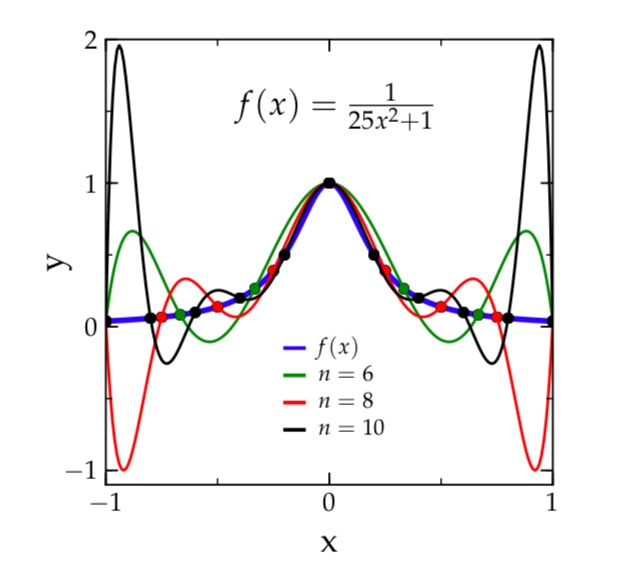
\includegraphics[scale=0.3]{interpolationExample.jpeg}
\end{figure}
\end{frame}

\begin{frame}[fragile]{Convergence of the Interpolated Function}
Data describe a continuous function $f(x)$ on an interval
$[a,b]$.\\
\pause
We expect that interpolating polynomials $p_n(x)$ with increasing degree $n$ make the interpolation
error converges to zero, i.e. \\
\begin{equation}
\lim_{n \to \infty} \left[ \max_{x \in [a,b]} |f(x) - p_n(x)|\right] = 0\,.
\end{equation} 
\pause

However,  for most continuous functions, this is not the case ! \\

\pause

This is called \emph{Runge's Phenomenon}. 
\end{frame}

\begin{frame}[fragile]{Lagrange Interpolation}
\begin{figure}
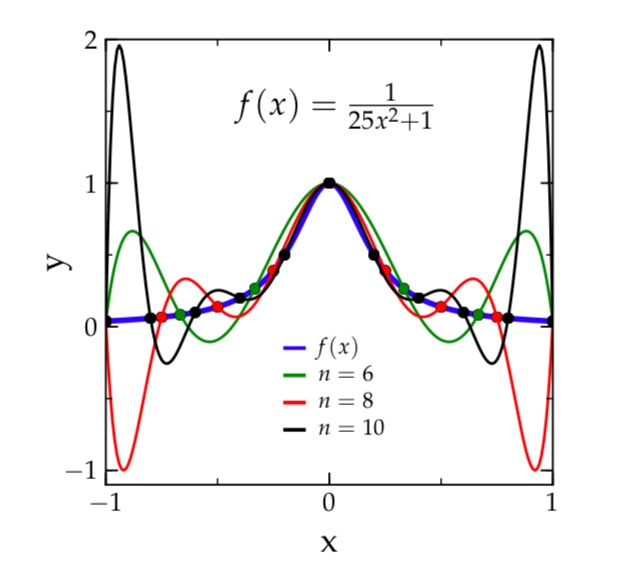
\includegraphics[scale=0.3]{interpolationExample.jpeg}
\end{figure}
\end{frame}


\begin{frame}[fragile]{Convergence of the Interpolated Function}

While the interpolating polynomials $p_n(s)$
converge to $f(x)$ near the peak, Runge's phenomenon produces strong oscillations and
divergences at the edges of the interval.

\bigskip

\pause
A higher polynomial degree could lead to a
greater error and unwanted oscillations!
\end{frame}

\begin{frame}[fragile]{Piecewise-polynomial Interpolation}

High degree polynomial interpolation should only be used
if one is certain that the function to be interpolated can be
approximated well globally by a single polynomial.
\bigskip
\pause

 If not, one can use \emph{piecewise-polynomial} interpolation. This uses
many low-degree polynomials instead of a single global polynomial.
\bigskip
\pause

The simplest form of piecewise polynomial interpolation is piecewise
linear interpolation ( connecting data points with straight
lines).
\end{frame}

\section{Hermite Interpolation}
\begin{frame}[fragile]{Hermite Interpolation}

Hermite interpolation is a form of polynomial interpolation in which
it is used data points as well as derivatives of the data. It reduces unwanted
oscillations (specially  if it is applied in piecewise form). \\
\bigskip
\pause

Now we will consider only the simplest case of Hermite
interpolation:  a function and its first derivative.\\
\pause

Consider $n+1$ data points. We will find a polynomial 
satisfying the conditions
\begin{equation}
p(x_i) = c_{i0}\,\,,\,\,\,p'(x_i) = c_{i1}\,\,\,\, \,\text{for}\,\,i \in [0,n]\,\,,
\end{equation}
where $c_{i0} = f(x_i)$ and $c_{i1} = f'(x_i)$.
\end{frame}


\begin{frame}[fragile]{Hermite Interpolation}
We propose the form
\begin{equation}
p(x) = \sum_{i=0}^n c_{i0} A_i(x) + \sum_{i=0}^n c_{i1} B_i(x)\,\,,
\end{equation}
where $A_i(x)$ and $B_i(x)$ are polynomials satisfying:
\renewcommand\arraystretch{1.2}%
\begin{equation}
\begin{array}{ll}
A_i(x_j) = \delta_{ij}\,\,,  &B_i(x_j) = 0\,\,,\\
A'_i(x_j) = 0\,\,, &B'_i(x_j) = \delta_{ij}\,\,.
\end{array}
\end{equation}
\renewcommand\arraystretch{1.0}%
\end{frame}

\begin{frame}[fragile]{Hermite Interpolation}
A possible form of the polynomials $A_i(x)$ and $B_i(x)$ is obtained using the Lagrange interpolation terms
\begin{equation}
L_{nj}(x) = \prod_{\substack{j = 0\\k\ne j}}^{n} \frac{x-x_k}{x_j - x_k}\,\,,
\end{equation}
as
\begin{equation}
\begin{array}{ll}
A_i(x) & = [ 1-2(x-x_i)L'_{ni}(x_i)]L_{ni}^2(x)\,\,,\\
B_i(x) & = (x-x_i) L_{ni}^2 (x)\,\,.
\end{array}
\end{equation}

\pause

Each $L_{ni}$ is of degree $n$ and therefore $A_i$ and $B_i$
are of degree $2n+1$ (The same as the maximal degree of $p(x)$). \\
\bigskip

\tiny
(see proof in
\url{http://www.math.umd.edu/~dlevy/books/na.pdf}. ) 

\end{frame}


\subsection{Piecewise Cubic Hermite Interpolation}
\begin{frame}[fragile]{Piecewise Cubic Hermite  Interpolation}
Consider a dataset such that for each point $x_i$
we also have the point $x_{i+1}$, as well as  the values $f(x_i)$, $f(x_{i+1})$, $f'(x_i)$, and
$f'(x_{i+1})$ (These values are known or can be evaluated numerically).

\bigskip
\pause

Taking $n=1$ in the Hermite interpolation equations we obtain  $A_i$ and $B_i$ as polynomials of degree $2n+1=3$.

\end{frame}

\begin{frame}[fragile]{Piecewise Cubic Hermite  Interpolation}
The cubic Hermite polynomial that interpolates $f(x)$ in $[x_i,x_{i+1}]$
is  given by
\begin{equation}
\begin{aligned}
H_3(x) =& f(x_i)\psi_0(z) + f(x_{i+1})\psi_0(1-z) \nonumber\\
& + f'(x_i)(x_{i+1} - x_{i})\psi_1(z) \nonumber \\ 
& - f'(x_{i+1})(x_{i+1}-x_i)\psi_1 (1-z)\,\,, 
\end{aligned}
\end{equation}
where 
\begin{align}
\psi_0(z) =&2z^3 - 3z^2 + 1\,\,,\\
\psi_1(z) =&z^3-2z^2+z\,\,.
\end{align}
and
\begin{equation}
z = \frac{x-x_i}{x_{i+1}-x_i}\,\,,
\end{equation}
\end{frame}

\section{Spline Interpolation}
\begin{frame}[fragile]{Spline Interpolation}
Splines are the ultimate method for piecewise polynomial interpolation.
It achieves smoothness by requiring continuity at
data points not only for the function values $f(x_i)$, but also for a
number of its derivatives $f^{(\ell)} (x_i)$. 
\bigskip
\pause

Assuming that we know the
values $f(x_i)$ at points $x_i$ ($i \in [0,n]$), we construct
piecewise polynomials of degree $m$ on each of the $n$ segments $[x_i,x_{i+1}]$,
\begin{equation}
p_i(x) = \sum_{k=0}^m c_{ik} x^k\,\,,
\end{equation}
to approximate $f(x)$ for $x \in [x_i,x_{i+1}]$. 
\end{frame}

\begin{frame}[fragile]{Spline Interpolation}
$m$ is the degree of the spline.\\
There are $m+1$ coefficients $c_{ik}$ for each $i$.\\
There are $n$ intervals.\\
\pause
\bigskip

Hence, there are $n (m+1)$ coefficients $c_{ik}$
that are determined by the conditions:
\begin{enumerate}
\item requiring $(n-1)(m-1)$ smoothness conditions at non-boundary
  points: $p_i^{\ell}(x_{i+1}) = p^{\ell}_{i+1}(x_{i+1})$ for $\ell=1,\cdots,m-1$,
\item requiring $2n$ interpolation conditions: $p_i(x_i) = f(x_i) =
  p_{i+1}(x_i)$,
\item choosing the remaining $m-1$ values of some of the $p_o^{\ell}(x_o)$
  and $p_{n-1}^{\ell}(x_n)$ for $\ell=1,\cdots,m-1$.
\end{enumerate}
\end{frame}

\subsection{Cubic Natural Spline Interpolation}
\begin{frame}[fragile]{Cubic Natural Spline Interpolation}
Consider $m=3$: Cubic Spline or \textit{Natural} Spline.\\ 
There are $m+1=4$ coefficients $c_{ik}$ for each $i$.\\
There are $n$ intervals.
\pause
\bigskip

Hence, there are $n (m+1)= 4n$ coefficients $c_{ik}$ and we need $4n$ conditions to find them and we need the information of the first and second derivatives.
\pause
\bigskip

The first choice is to set the highest derivative to zero on both ends of the interval:
\begin{equation}
p''_0(x_0) = 0\,\,,\,\,\,p''_{n-1} (x_n) = 0\,\,.
\end{equation}
\end{frame}

\begin{frame}[fragile]{Cubic Natural Spline Interpolation}
Then we consider the linear
interpolation of the second derivative in $[x_i,x_{i+1}]$,
\begin{equation}
p_i''(x) = \frac{1}{x_{i+1}-x_i} \left[ (x-x_i)p''_{i+1} - (x-x_{i+1})
  p''_i \right]\,\,,
\end{equation}
where $p_i'' = p_i''(x_i) = p_{i-1}''(x_i)$ and
$p''_{i+1} = p''_{i+1}(x_{i+1}) = p_i''(x_{i+1})$.
\end{frame}

\begin{frame}[fragile]{Cubic Natural Spline Interpolation}
Integration of this interpolated second derivative two times and using $f_i =
p_i(x_i) = f(x_i)$ gives
\begin{equation}
p_i(x) = \alpha_i (x-x_i)^3 + \beta_i (x-x_{i+1})^3 + \gamma_i (x-x_i) + 
\eta_i(x-x_{i+1})\,,
\end{equation}
where
\begin{align}
\alpha_i &= \frac{p_{i+1}''}{6 h_i} &\beta_i &= \frac{-p_i''}{6h_i}\,,\\
\gamma_i &= \frac{f_{i+1}}{h_i} - \frac{h_i p''_{i+1}}{6}
&\eta_i &= \frac{h_i p_i''}{6} - \frac{f_i}{h_i}\,\,,
\end{align}

with $h_i = x_{i+1} - x_{i}$. 
\pause
\bigskip

Hence, all we need to find the spline is
to know all of its second derivatives $p_i'' = p_i''(x_i)$.
\end{frame}

\begin{frame}[fragile]{Cubic Natural Spline Interpolation}
Now apply the condition $p_{i-1}'(x_i) = p_i'(x_i)$ to the interpolated polynomial to obtain the equation
\begin{equation}
h_{i-1}p_{i-1}'' + 2 (h_{i-1} + h_i)p_i'' + h_i p_{i+1}'' = 
6 \left( \frac{g_i}{h_i} - \frac{g_{i-1}}{h_{i-1}}\right)\,\,,
\end{equation}
where $g_i = f_{i+1} - f_i$.\\
\pause
\bigskip
 
This is a linear system with $n-1$ unknowns:
$p''_i$ for $i=1,\cdots,n-1$ ( remember that $p_0'' = p_n'' = 0$, as set by the natural
spline condition.
\end{frame}

\begin{frame}[fragile]{Cubic Natural Spline Interpolation}
Defining $d_i = 2(h_{i-1} + h_i)$ and $b_i = 6\left(\frac{g_i}{h_i} 
- \frac{g_{i-1}}{h_{i-1}}\right)$, we can write 
\begin{equation}
A p'' = b \hspace{1em}\text{ with } A_{ij} = \left\{ \begin{array}{ll}
d_i &\text{if } i=j\,,\\
h_i &\text{if } i=j-1\,,\\
h_{i-1}&\text{if } i=j+1\,,\\
0&\text{otherwise}.
\end{array}\right.
\end{equation}
\pause

The coefficient matrix $A_{ij}$ is real, symmetric, and tri-diagonal.\\
The solution of such a linear system of equations will be presented later in the course.
\end{frame}

\end{document}